\section{Leads before \passage{Balamory}}

When James and I went to have a look at the bottom of \passage{Balamory} on
the first day of our one-night camping trip, we didn't make it to the
target as an unexpected first pitch used up too much of the rope that we
had taken with us.

\margininbox{2-8 10:20am}{

Good night's sleep in the old `buff bag' -- nice to think I was sleeping
in the same bag that we used at the \passage{Hotel} in 1998! Camp \passage{X-Ray} is
becoming more like home. \name{Tetley}
\textit{23:58} --
Karin and I had a great day looking at all the new finds beyond \passage{Leopard}.
I put 3 more bolts on \passage{Cheetah} pitch plus deviation. We looked in
vain for more easy horizontal passage. Hopefully Tjaša, Erik, Izzy and
Mawr have more luck. Time for sleep now -- James and Dave complete the 4
bed camp.\name{Tetley}}{\logbook}

However, as well as airflow going towards \passage{Balamory}, there is also
airflow in the main passage above, beyond the point where the hole down
to \passage{Balamory} leads off so here are two leads in that area there
that are worth looking at.

The upper lead does need some way of climbing across a pit to a
ledge covered in loose crap (maybe a bolt traverse round one of the
walls, though I can't remember how much good rock there was in that
area).

Subsequent email exchanges on the subject do seem a bit vague as to
exactly what was done, and whether the upper passage had actually been
boldly examined or not (Clewin was bold somewhere round there, but it
wasn't certain where), but anyone going to potentially move/split the
boulder down \passage{Balamory} (I think it was supposed to be down the
third of the three possible `second pitches') down should also probably
plan to look at the upper passage continuation, especially if they have
a drill/bolts to help with climbing/traversing belays.

It was on the way back from this little trip, after grabbing some stashed
karrimats from the old camp, that the black black hole across \passage{Big
Rock Candy Mountain} was noticed\sidenote{see 2012 expedition}.
\name{Dave Wilson}

\subsection{Pushing Hidden Surprise and finding Kamikaze}


The next day, James and I went to the new stuff below
\passage{Leopard} / \passage{Cheetah}, but since we were doing a push-then-out
trip, rather than going to the far end of the `half' where most of the
action was, we went in the other direction from the pitch bottom to do
some work relatively close to camp, carrying on where Gergely and company had
left off at the \passage{Hidden Surprise} pitch.

    \begin{marginfigure}
\checkoddpage \ifoddpage \forcerectofloat \else \forceversofloat \fi
\centering
 \frame{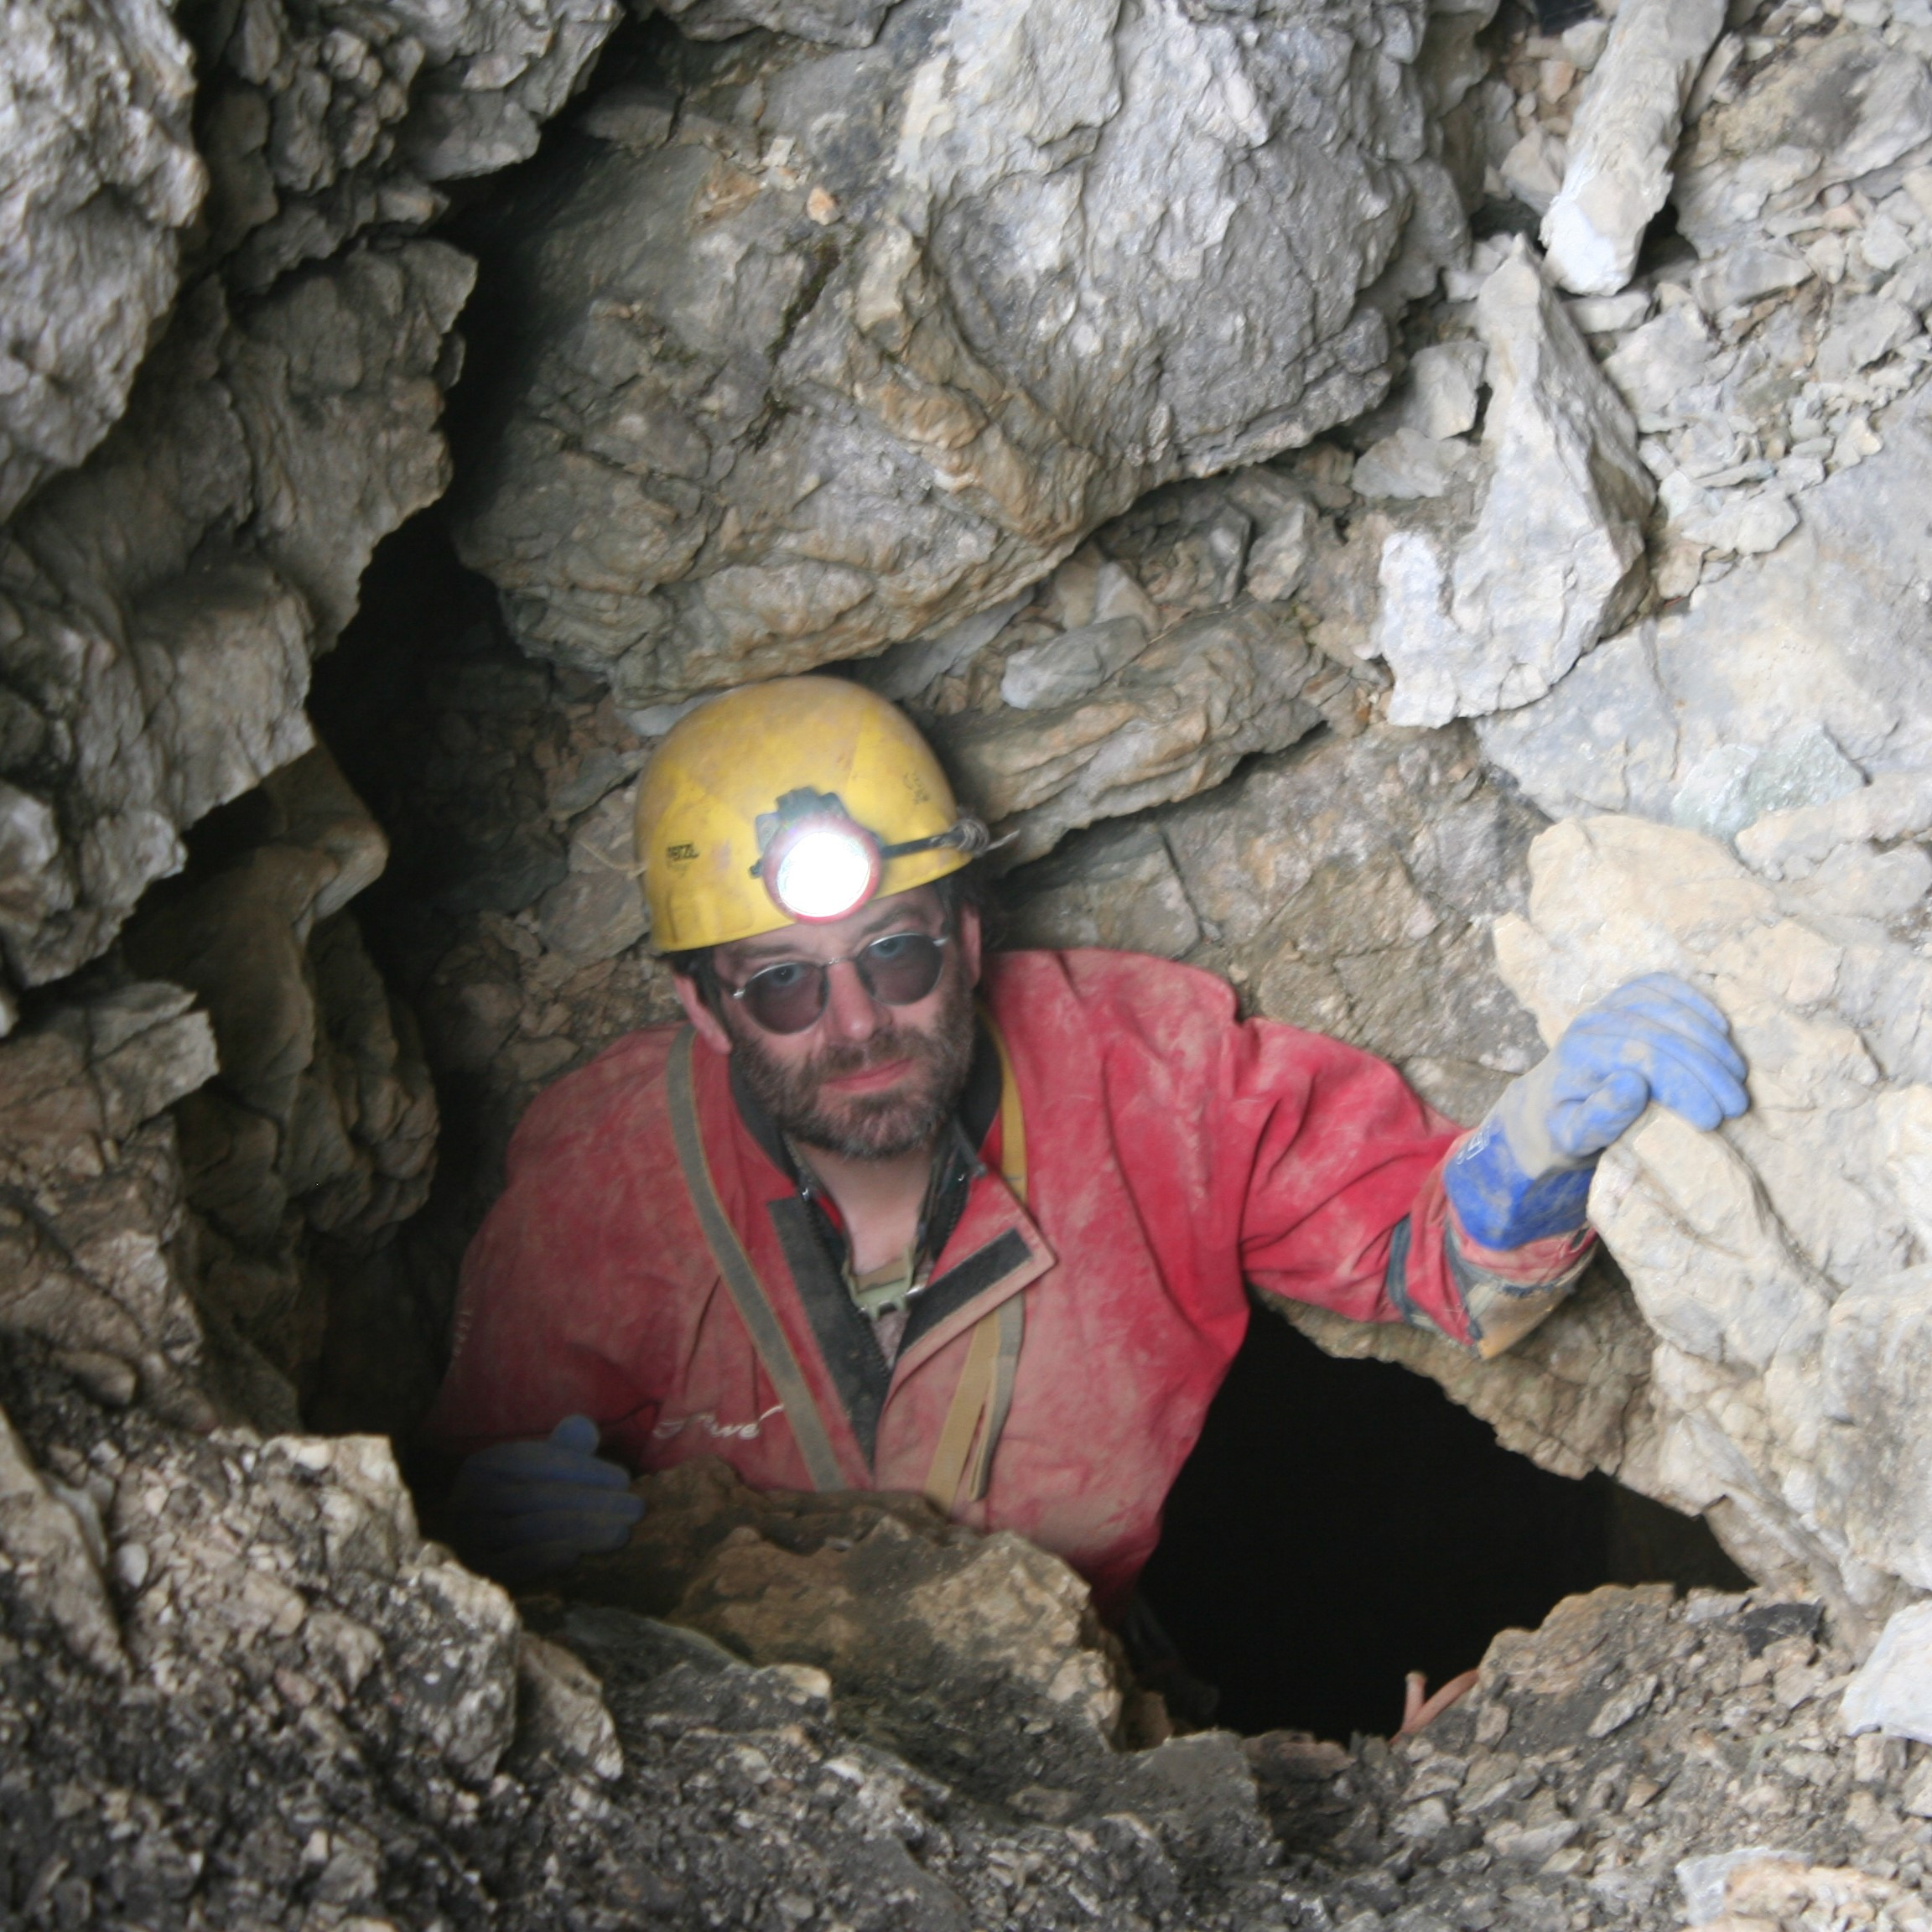
\includegraphics[width=\linewidth]{2010/balamory/20100810-11-25-27 - Jana Carga 43--orig.jpg}} 
 \caption{Dave entering \protect\passage{Vrtnarija}. \pic{Jana Čarga}}
 \label{dw gw}
\end{marginfigure}

Gergely had dropped the first section of the pitch to an obvious ledge
and followed the ledge to horizontal passage that soon died. James and I
were to descend the shaft from the ledge, but it immediately became
clear the drill wasn't working and so we had to resort to spits, with
James bolting while I waited on the ledge.

Fairly soon the bolt (bolts?) was in and James had descended to a large
boulder-covered ledge part-way down the large shaft, where I could
safely join him. Some of the boulders were rather large, with gaps
between them or between them and the wall large enough to climb down and
move around in. While James did the business with the next spit, I
wandered around between the boulders to keep busy. Where the boulders
met the wall, the wall was somewhat overhanging, and from the lowest
easily-accessible place near where I had first climbed down, it was
possible to look between the boulders marking the lower limit of easy
movement and the wall to see a few metres away/down to where the wall
seems to meet the proper floor of the ledge, where there was a layer of
white rock flour, with some potentially human-sized space between me and
it though with no obvious way to get there.


\margininbox{Kamikaze}{
     \begin{itemize}
    \item James Kirkpatrick
    \item Dave Wilson
    \end{itemize}}{\explo}


From where I was, looking along the wall `clockwise', it also looked
like there was a space of some sort ahead of me horizontally, but
getting to it didn't look very nice, and after all, I was just in a pile
of boulders on a big ledge half-way down a pitch, not in a classic
boulder choke as such, so there seemed little point doing anything
borderline just to get to a slightly different place in the boulder
pile.

However, just as I was preparing to go back up and see how James was
getting on, I breathed out a large sigh, only to see it get sucked
horizontally away from me between wall and boulders and into the space I
had been looking into, which immediately aroused my curiosity.


\begin{pagefigure}
\checkoddpage \ifoddpage \forcerectofloat \else \forceversofloat \fi
\frame{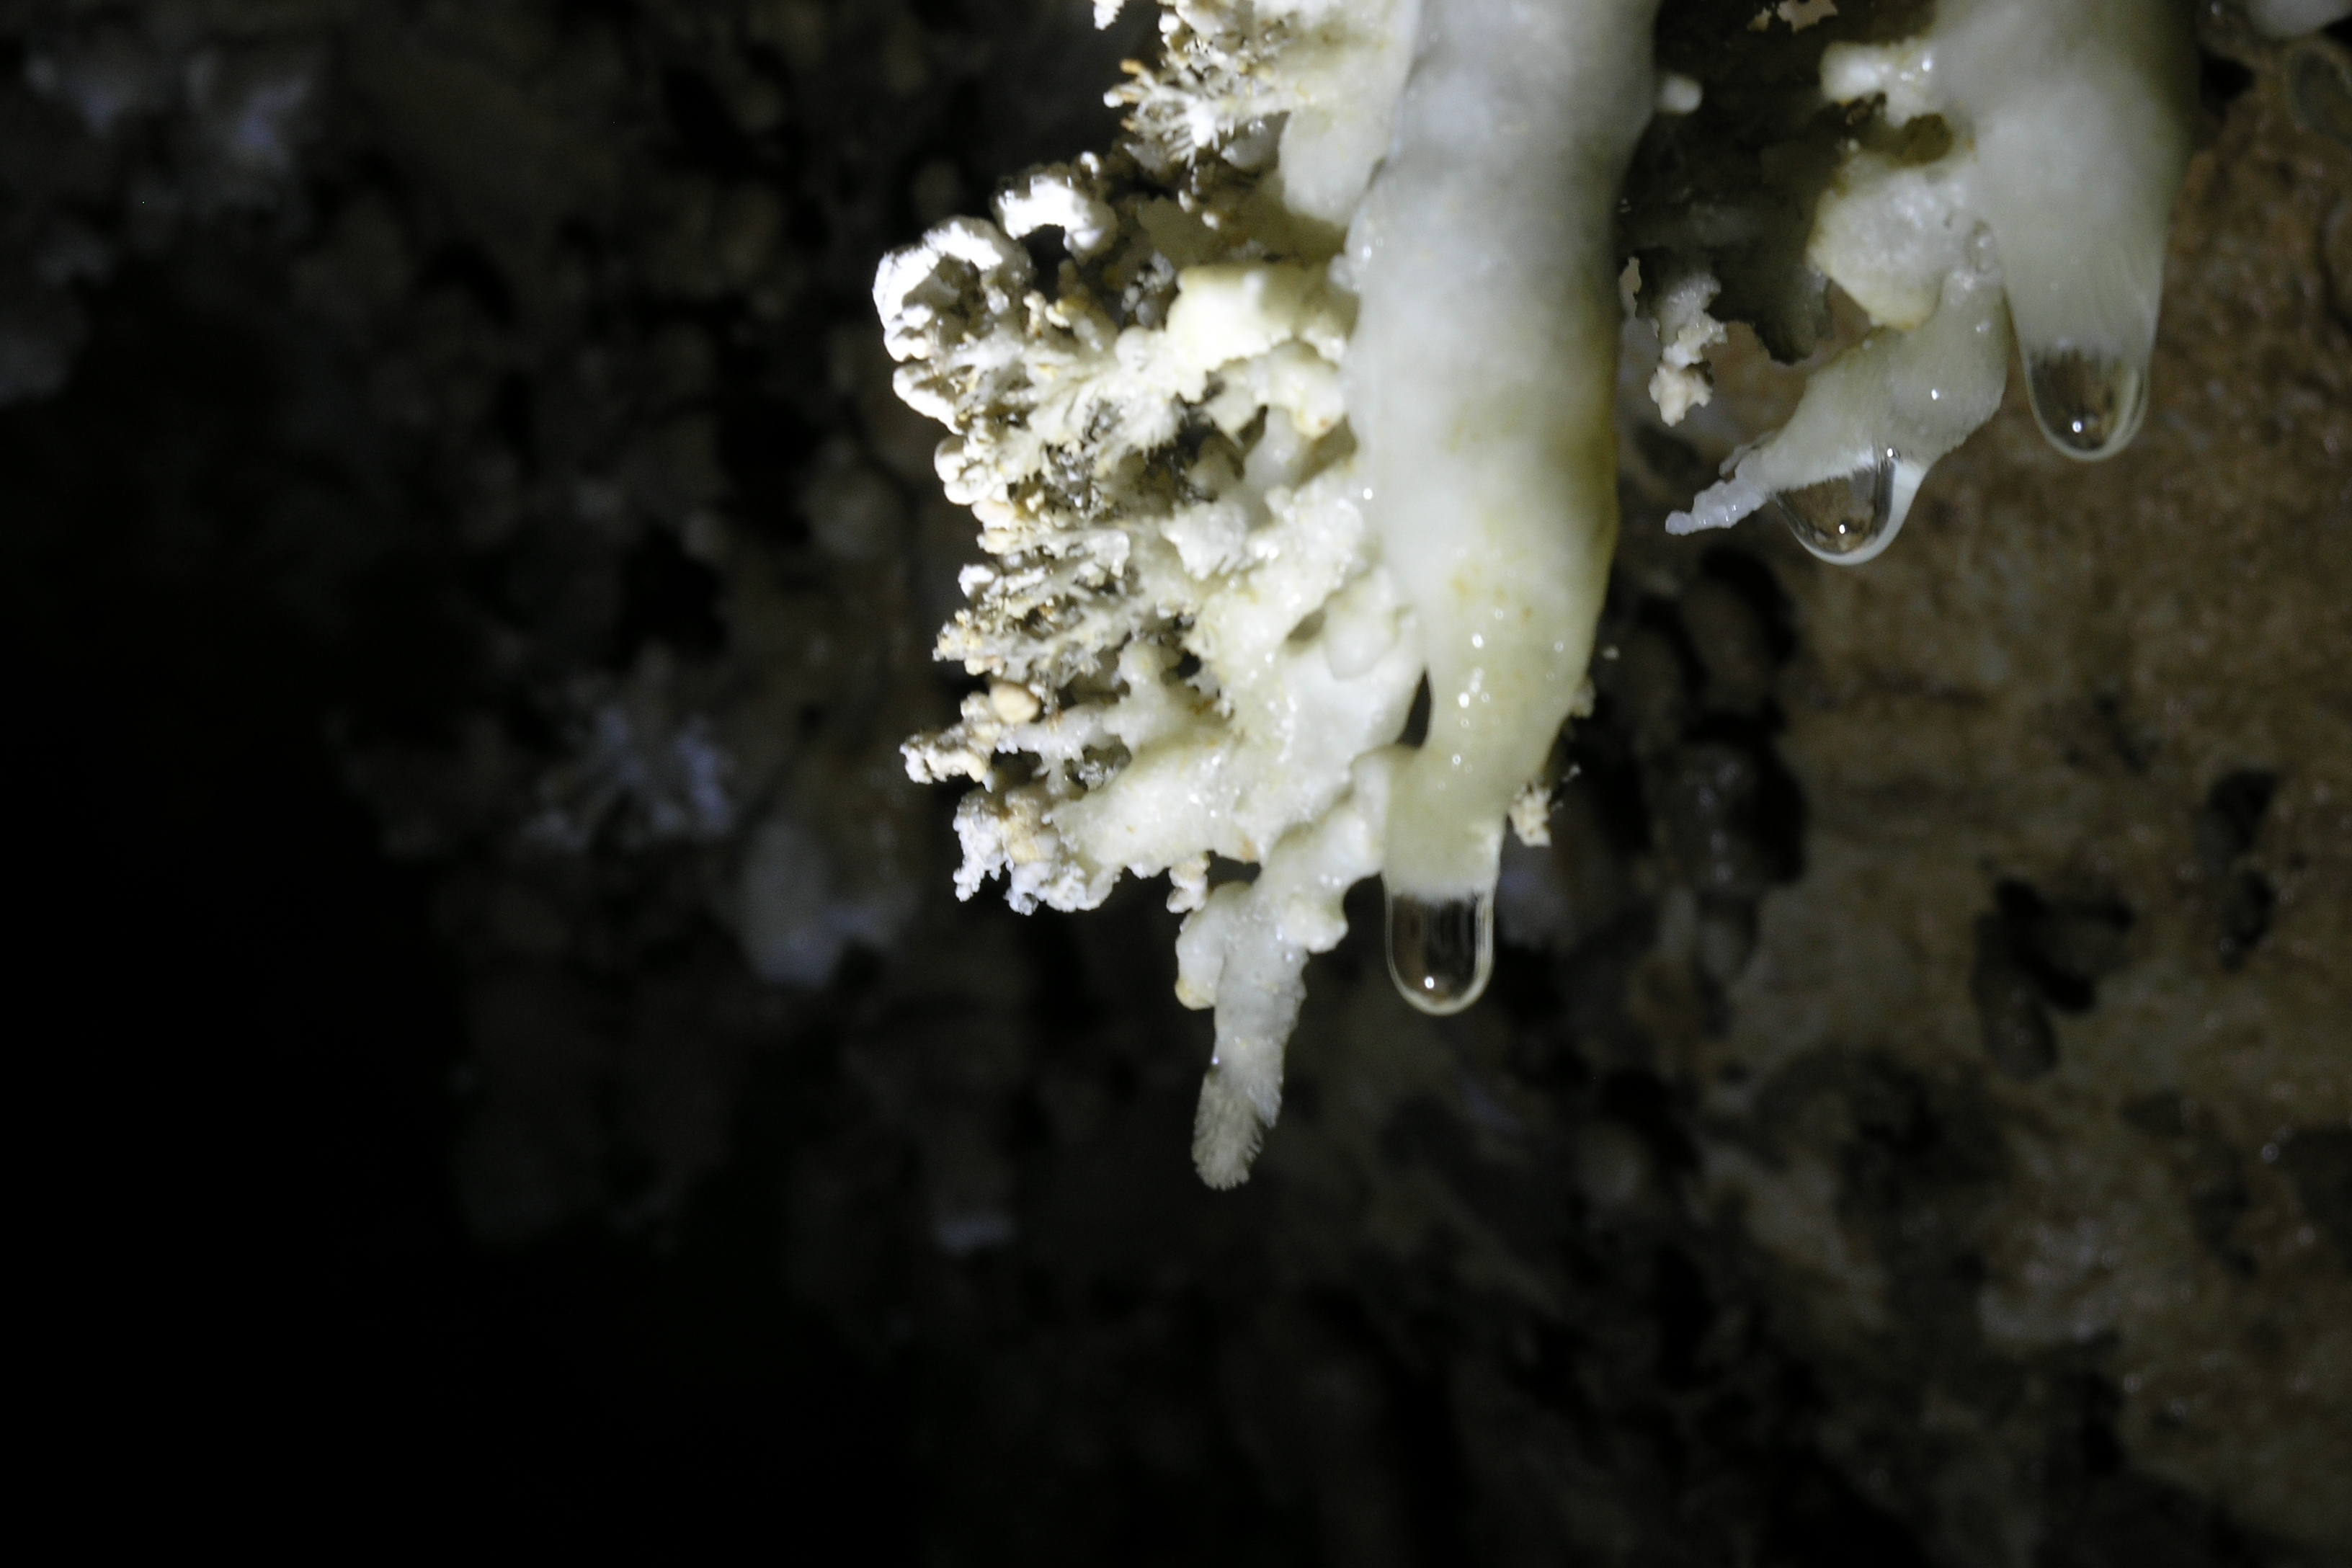
\includegraphics[width=\linewidth]{2010/balamory/20100804-19-31-07 - Nikolas Kral - P8041834 - Formations at bottom of Cheetah--orig.jpg}}
\caption{One of the formations at the base of \protect\passage{Cheetah} pitch. \pic{Nikolas Kral}}
\end{pagefigure}


To get into the space I could see required going horizontally through a
not-quite-body-sized vertically-rectangular gap with a 1 m drop on the other side. After removing all my SRT kit, and doing some work
with a convenient rock hammering edges off the boulder forming one side
of the slot to make the gap wider, and progressively blunting sharp
edges on the wall side as they proved awkward when attempting to get
through, it was possible to slowly and delicately post myself through
feet first and eventually emerge free on the other side.



\begin{figure*}[t!]
\checkoddpage \ifoddpage \forcerectofloat \else \forceversofloat \fi
\frame{\includegraphics[width=\linewidth]{2010/balamory/20100731-20-27-46 - Martin McGowan Canon 50D - IMG_1524 - Crystal Hall in Palace of King Minos--orig.jpg}}
\caption{Crystals in the \protect\passage{Palace of King Minos}, in an area nicknamed 'Crystal Hall'. \pic{Martin McGowan}}
\end{figure*}


Turning around, a short crawl led to a wider area under the overhanging
wall, and a view ahead to where the wall/roof sloped nicely down towards
into the floor to leave a wide bedding plane with clearly no way on.
Turning around somewhat disappointed, the main wall, which I had been
looking away from when I had initially turned round, was seen to have a
crawling-height hole in it, which, on approaching, it was clear most of
the draught was going into.

That hole led to a small chamber with a further hole leading in turn
into the side of a walking-height passage with a good breeze running
along it. The draught I had followed initially was clearly just a
tributary being sucked into the main airflow.

I quickly returned to James to tell him of the find, and we decided to
do a little surveying and exploration. We chose the upwind branch which
didn't run a great distance before ending in an upwards bedding-plane
slope ultimately blocked by a large slab in the bedding blocking
sideways movement into what appeared to be a chamber with a waterfall
entering. Capping or plugs/feathers would seem to be needed to shift
this blockage. On returning to our entry point, we looked the other way,
wondered how far the downwind passage went, but left it for someone else
to explore.

We hadn't found a great deal of length, but on the other hand, we had
left a decent going lead, and due to the combination of a misbehaving
drill making waiting cold and dull work and the luck of my breath
showing there was something worth looking at, had ended up finding quite
interesting passage in what must be one of the most unlikely of
situations.

    \begin{marginfigure}
\checkoddpage \ifoddpage \forcerectofloat \else \forceversofloat \fi
\centering
    \frame{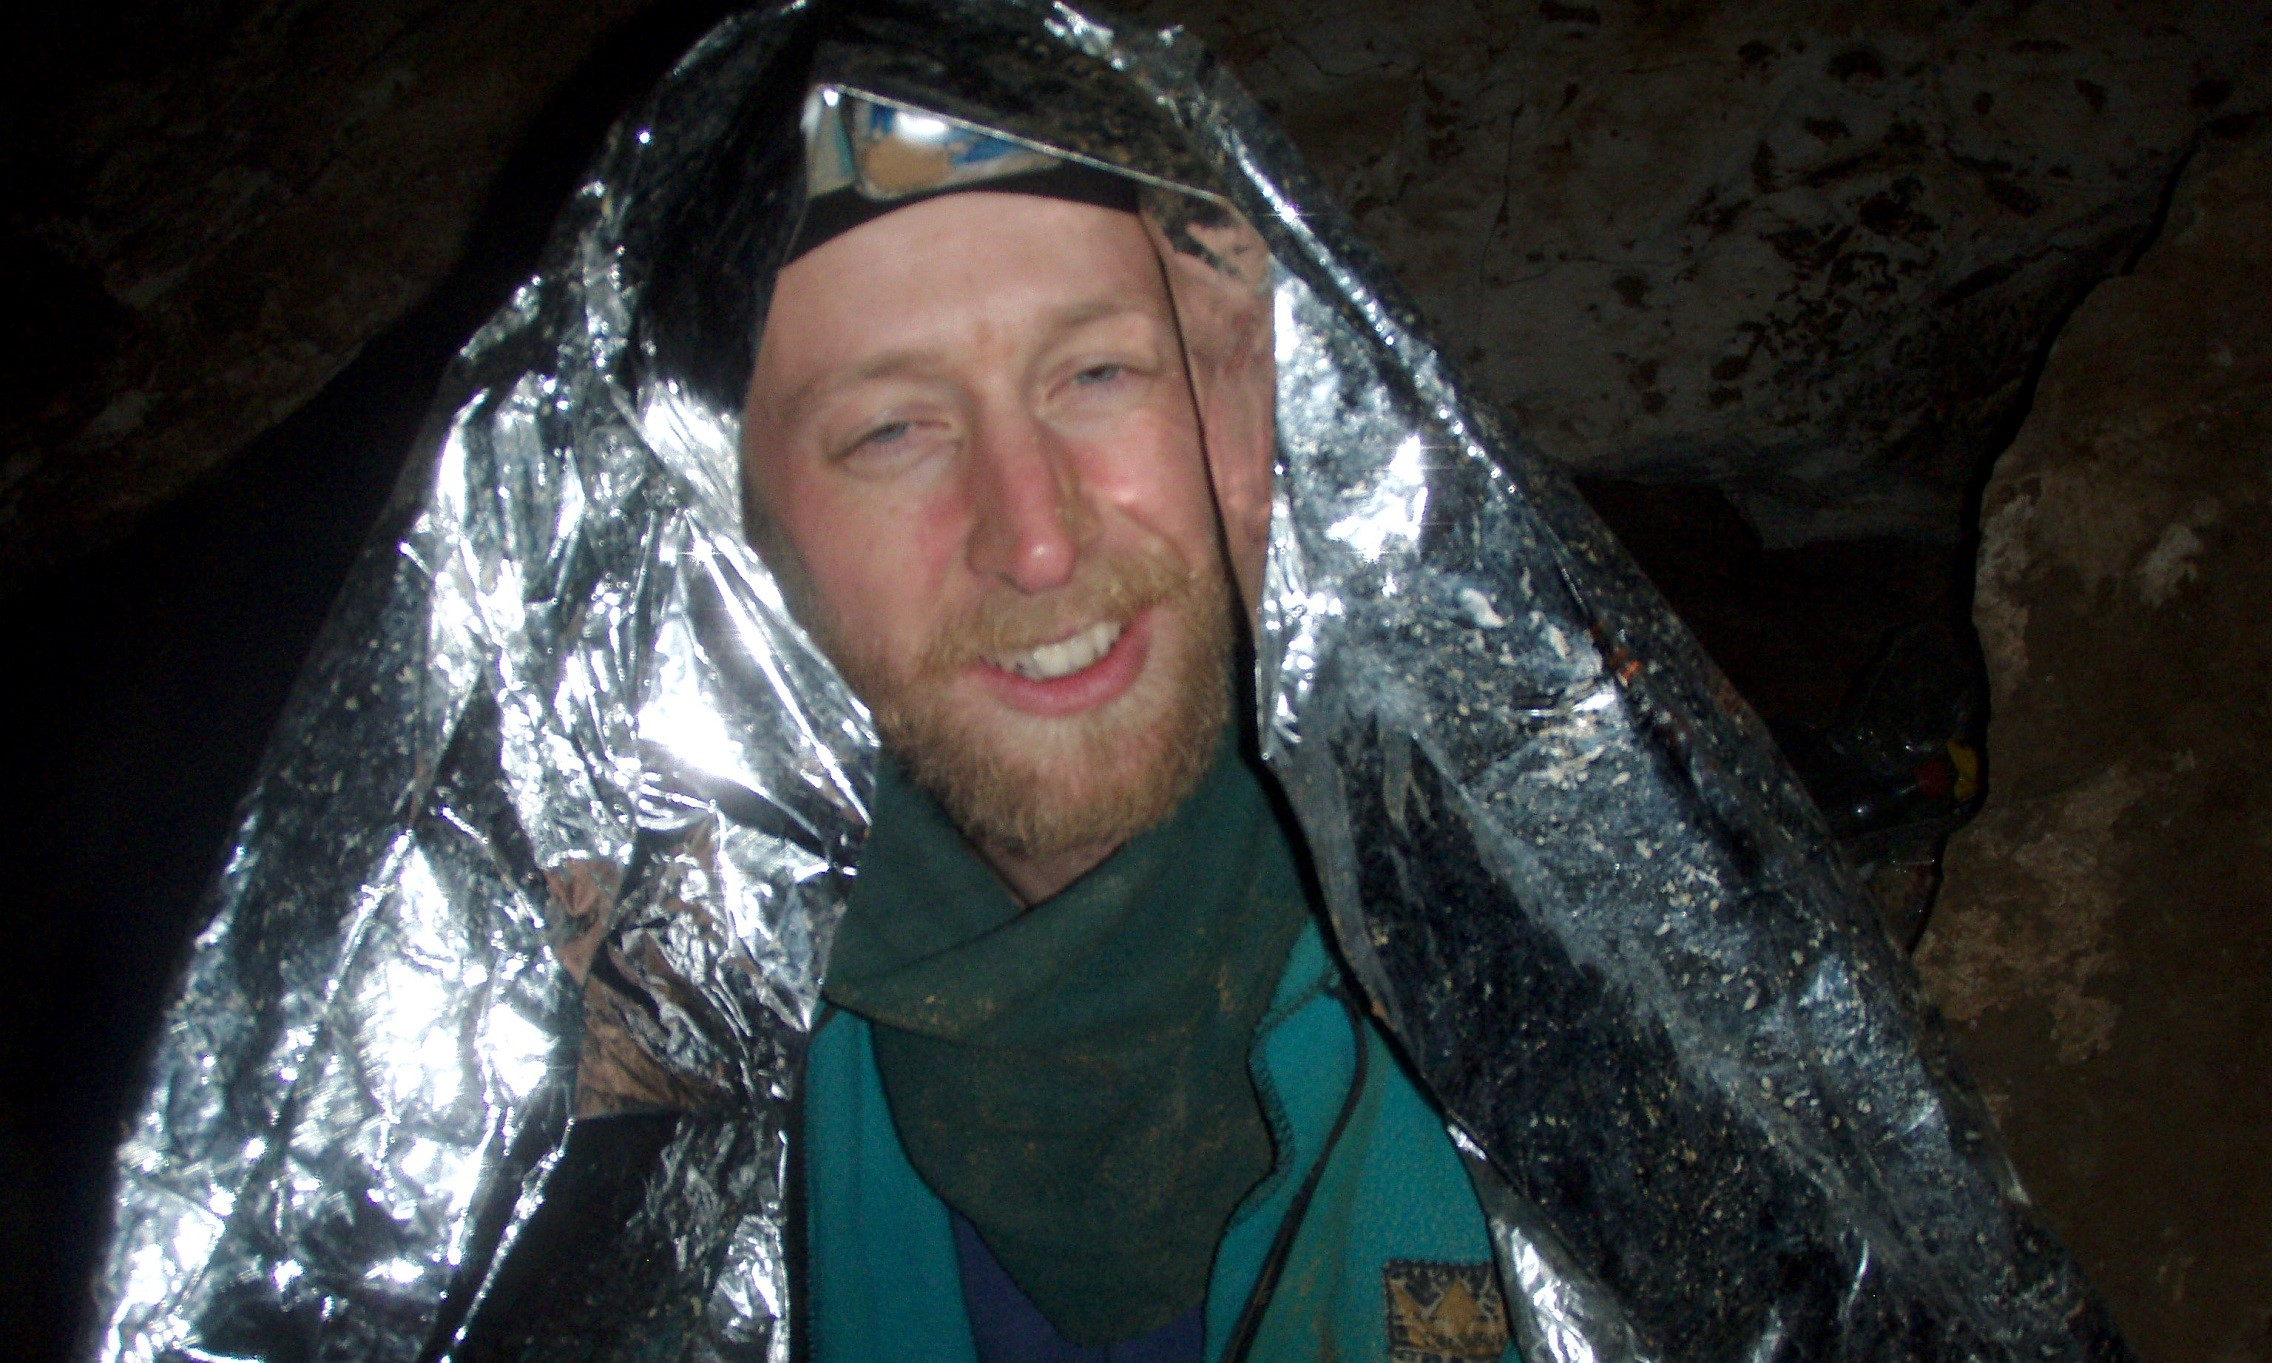
\includegraphics[width=\linewidth]{2010/balamory/20100806-02-48-30 - Jan Evetts - P2060080 - Camp X-ray--orig.jpg}}
 \caption{Jan keeping warm under a foil blanket at camp \passage{X-ray}. \pic {Jan Evetts}}\label{foil xray}
\end{marginfigure}

Thinking partly of the initial nervousness with which I had slowly
posted myself between the boulders and the wall, but mainly of the
immense luck we had had with the draught, \passage{Kamikaze} seemed like
the obvious choice of name for the discovery.

\name{Dave Wilson}


\fullwidthbox{5-8-10 - Thara and Niko's \passage{Lost Hopes}}{

Left for \passage{Kamikazi} pushing front. Rigged down the 10 m pitch. At the
bottom, there is a flowing passage which will be big enough for humans
in 1 million years. About 1 m above the bottom there is a window which
turns out to be a lot of crawling/squeezes. There are two small chambers
along the way for us to stand. At the second chamber we climber down
into active water passage. Upstream is dead but downstream is blocked by
a squeeze worthy of Jana. We left unsurveyed as we forgot the tape. Next
we checked the window at the level of deviation. Same thing. It kept
going and the gap on Nico's oversuit widen to cover both buttocks. On
the way out of the window, I heard a sudden change in water flow. It
must be raining outside 8 hrs before. (This was at 7pm). Surveyed in wet
conditions was not fun!
\name{Thara Supasiti}}


    \begin{figure*}[b!]
\checkoddpage \ifoddpage \forcerectofloat \else \forceversofloat \fi
\centering
  \frame{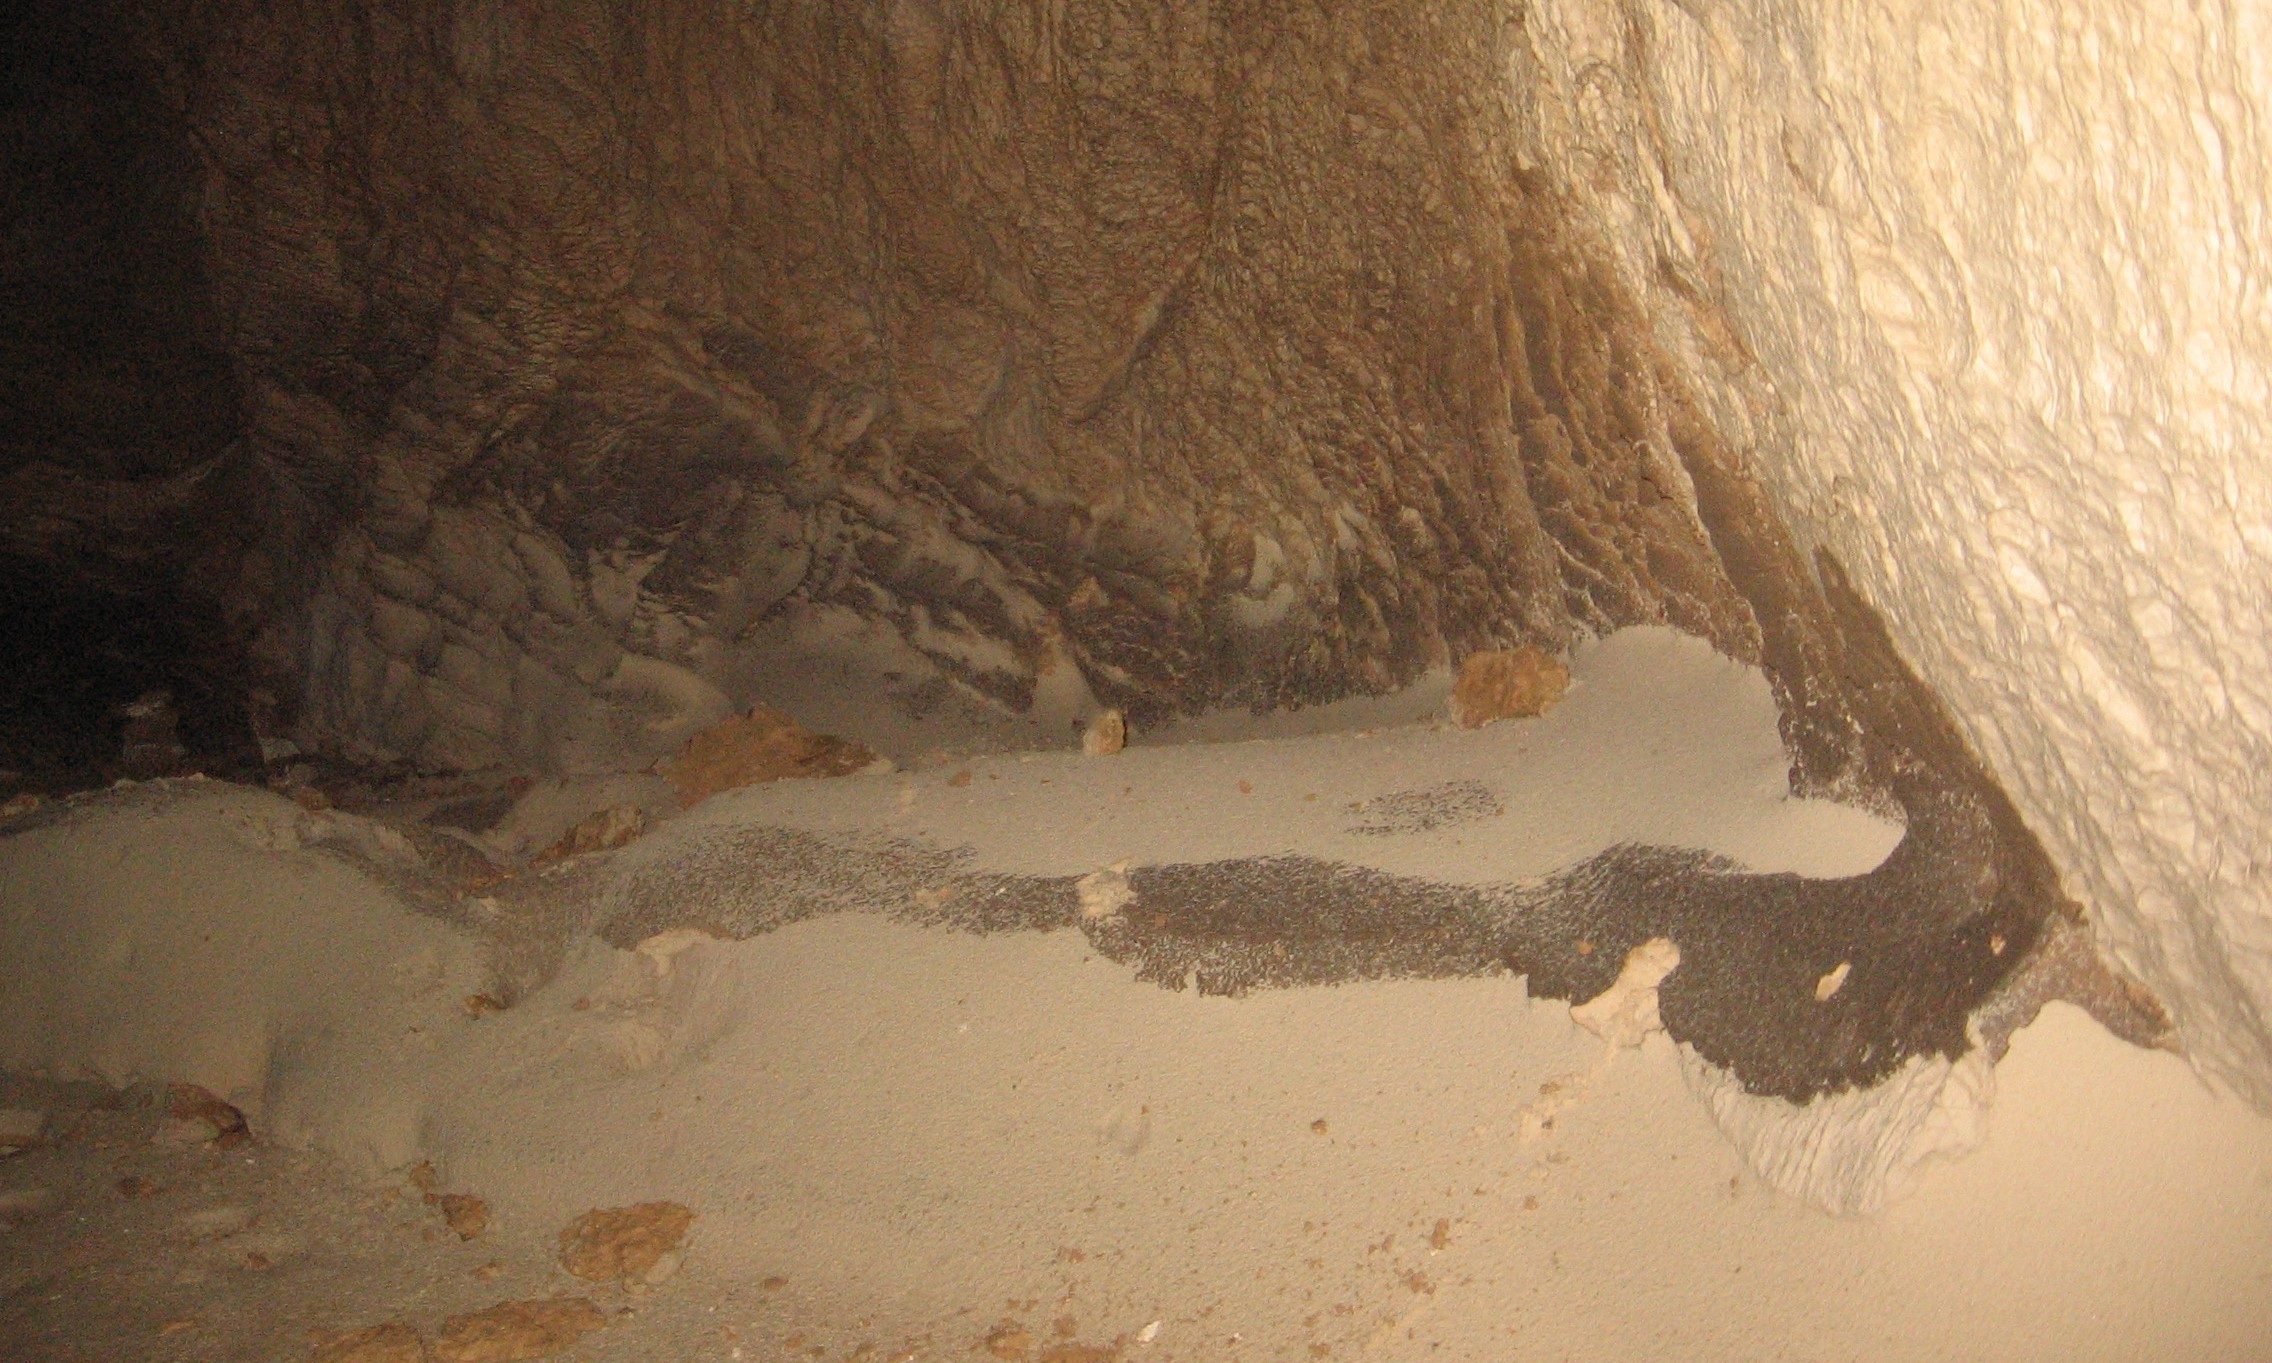
\includegraphics[width=\linewidth]{2010/balamory/20100809-17-54-38 - Jarvist Frost A520 - IMG_0024 - Lost Hopes Inlet ledge--orig.jpg}} 
        \caption{Inlet ledge in \protect\passage{Lost Hopes}, below \protect\passage{Kamikaze}. \pic {Jarvist Frost}} \label{lost hopes inlet}
\end{figure*}


